%%%%%%%%%%%%%%%%%%%%%%%%%%%%%%%%%%%%%%%%%%%%%%%
%%%%%%%%%%%%%%%%%%%%%%%%%%%%%%%%%%%%%%%%%%%%%%%
\subsection{Dark Matter signatures and rates}
The i2HDM exhibits various signatures that are potentially accessible at the LHC.
First of all, it provides  a mono-jet signature from the $pp\to h_1 h_1j$ process,
the Feynman diagrams for which are presented in Fig.~\ref{fig:fd-monojet1}.
\begin{figure}[htb]
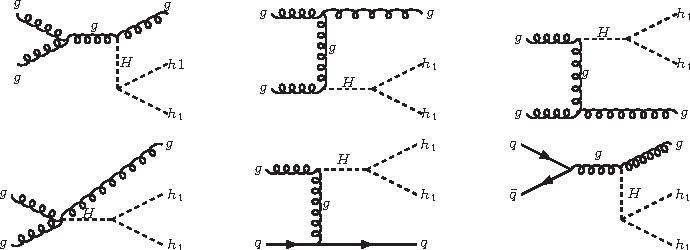
\includegraphics[width=\textwidth]{Figures/fd-mono-j1.pdf} 
\caption{Feynman diagrams for the $pp\to h_1 h_1j$ process
contributing to a mono-jet signature.}
\label{fig:fd-monojet1}
\end{figure}
For this process, the relevant non-trivial  parameter space is  one dimensional:
it is just the DM mass, $M_{h_1}$,  since the second parameter, $\lambda_{345}$,
simply scales the production cross section which is proportional to  $(\lambda_{345})^2$
for $M_{h_1}>M_H/2$.
One should note  that the mediator mass for this signature is the Higgs mass, $M_H = 125$ GeV, thus
the Effective Field Theory (EFT) approach is not applicable for this process. Also, the recent limits by ATLAS
\cite{Diehl:2014dda} and CMS \cite{Chatrchyan:2012me, Khachatryan:2014rra} collaborations  are not directly
applicable for this process since they have been obtained for a different spin of the mediator and different
spin of DM. 

There is one more process, namely $q\bar{q}\to
h_1 h_2g$ ($gq\to h_1 h_2q$) (see diagrams in 
Fig.~\ref{fig:fd-monojet2}),  that can contribute to a mono-jet signature in the special case of a small mass split between $h_1$ and $h_2$.
In this scenario $h_2$ decays to $h_1$ plus soft 
jets and/or leptons. 
\begin{figure}[htb]
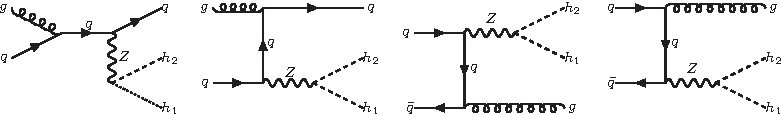
\includegraphics[width=\textwidth]{Figures/fd-mono-j2.pdf} 
\caption{Feynman diagrams for $q\bar{q}\to h_1 h_2g$ ($gq\to h_1 h_2q$) process 
contributing to mono-jet signature.}
\label{fig:fd-monojet2}
\end{figure}
%In spite of the fact that there is one mediator for this process -- the $Z$-boson --
%one can see that $t-$ and $s-$channel topologies with a light quark in the propagator 
%make this process different from simplified models with fermion dark matter and vector mediator, which have
%been  studied so far\giac{[Add references]}{}. 
The essential parameter space for this process is the
two-dimensional  ($M_{h_1},M_{h_2}$) plane
which fixes its cross section.

Besides mono-jets, the i2HDM gives rise to a mono-$Z$ signature, the 
diagrams for which are presented in Fig.~\ref{fig:fd-mono-Z}.
The first diagram scales with $\lambda_{345}$ while the other two are fixed by electroweak interactions.\footnote{For the second diagram, the $ZZh_1h_1$ vertex for transverse $Z$-bosons is fixed by the weak coupling,
while for longitudinal $Z$-boson it scales with with $\tilde\lambda_{345}$ in Eq.~(\ref{tildelam345}). 
When this coupling is small, the strength of the  $ZZh_1h_1$ vertex therefore
is fixed by the gauge interactions.}
In general, non-trivial interference takes place between the three different topologies represented by each of three 
diagrams, so  this process cannot be approximated by a simplified model.
However, we found that when $|\lambda_{345}|\gtrsim 0.02$ with $M_{h_1}< M_H/2$ (below the Higgs boson threshold)
or $|\lambda_{345}|\gtrsim 1$ with $M_{h_1}> M_H/2$ (above the Higgs boson threshold),
the first diagram is dominant and defines the event kinematics. 
So for these values of $\lambda_{345}$ and $M_{h_1}$, a simplified
model with the Higgs boson as the mediator is sufficient to set the LHC limits.

One should also note that for values of $|\lambda_{345}|$
below $0.02$ the contribution from diagrams scaling with $|\lambda_{345}|$
drops below $1\%$. In this case the
$Z$ boson will be the only mediator to probe the i2HDM model at the LHC,
with the mono-$Z$ process being the leading signature
for this purpose (and not only as a probe complementary to the mono-jet signature). 
This signature will be especially pronounced if $M_{h_2}-M_{h_1} > M_Z$,
so that the cross section of the mono-$Z$ signature
is essentially defined by the cross section of the $2 \to 2$ process,
$pp\to h_1 h_2 \to h_1 h_1 Z$.
The parameter space for this process is
the two-dimensional $(M_{h_1},M_{h_2})$ plane.
%
\begin{figure}[htb]
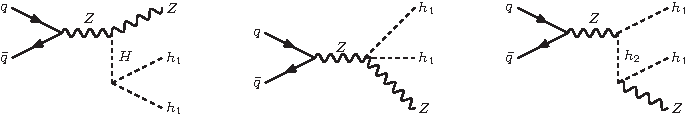
\includegraphics[width=\textwidth]{Figures/fd-mono-z.pdf} 
\caption{Feynman diagrams for $q\bar{q}\to h_1 h_1Z$  process 
contributing to mono-Z signature.}
\label{fig:fd-mono-Z}
\end{figure}
%

The i2HDM could also provide a mono-Higgs signature
via $gg\to  h_1 h_1 H$ and $q\bar{q} \to  h_1 h_2H$,
whose diagrams are presented in Fig.~\ref{fig:fd-mono-H1}
and Fig.~\ref{fig:fd-mono-H2} respectively.
%
\begin{figure}[htb]
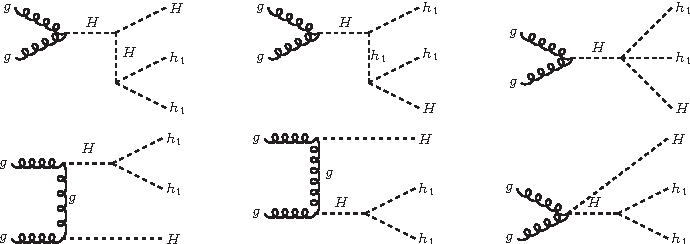
\includegraphics[width=\textwidth]{Figures/fd-mono-h1.pdf} 
\caption{Feynman diagrams for $gg\to h_1 h_1H$  process 
contributing to mono-Higgs signature.}
\label{fig:fd-mono-H1}
\end{figure}
\begin{figure}[htb]
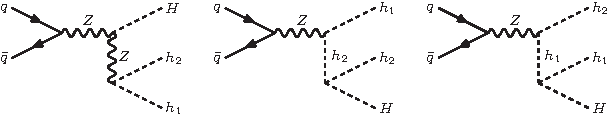
\includegraphics[width=\textwidth]{Figures/fd-mono-h2.pdf} 
\caption{Feynman diagrams for $q\bar{q}\to h_1 h_2H$  process 
  contributing to mono-Higgs signature.}
\label{fig:fd-mono-H2}
\end{figure}
The only mediator for $gg\to  h_1 h_1 H$ is the Higgs boson,
and the respective cross section scales as $(\lambda_{345})^2$
for small values of $\lambda_{345}$ 
and $(\lambda_{345})^4$ for large values of $\lambda_{345}$
because of the second diagram.
On the other hand, the $q\bar{q}\to h_1 h_2H$  process 
takes place via either a $Z$-boson or an $h_2$ as a mediator:
the first diagram does not scale with $\lambda_{345}$,
while the last two do. Therefore for large $\lambda_{345}$,
the $(\lambda_{345})^2$  scaling takes place for $q\bar{q}\to h_1 h_2H$ process.
In fact,  the contribution from the second and 
the third  diagrams of  $q\bar{q}\to h_1 h_2H$
to the total cross section
drops below 1\% only for $\lambda_{345}<0.002$,
below which the process kinematics and the cross section 
are determined by the first diagram with two $Z$-boson propagators.

\begin{figure}[htb]
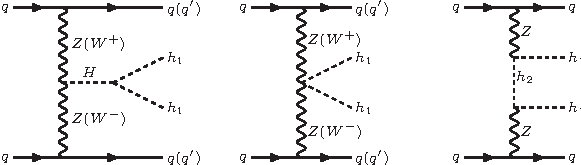
\includegraphics[width=\textwidth]{Figures/fd-vbf.pdf} 
\caption{Diagrams for $qq\to q^{(')}q^{(')} h_1 h_1$ DM production in vector boson
  fusion process.}
\label{fig:fd-vbf}
\end{figure}
%
Finally, one should mention the production of DM via vector boson fusion, $pp\to h_1 h_1 jj$, the diagrams for which are
presented in Fig.~\ref{fig:fd-vbf}.
Similarly to the mono-$Z$ process, there are three diagrams with different
topologies and mediators which contribute to this process; thus,
it cannot be described by  just one simplified model.
The first two diagrams scale with $\lambda_{345}$.
To be accurate, the $Z_L Z_L h_1 h_1$ coupling in the second diagram is proportional to 
$\tilde\lambda_{345}$, see Eq.~(\ref{tildelam345}), which is approximately equal to $\lambda_{345}$ for small 
$M_{h_2}-M_{h_1}$.
They give the dominant contribution to the  $pp\to h_1 h_1 jj$ process for $\lambda_{345}\simeq 1$,
but their contribution is negligible with very small $\lambda_{345}$.
%which decouples  only for  $\lambda_{345}\lesssim 1$,
%when  the contribution from the first two diagrams drops below the per-cent level.
On the other hand, for large $h_1-h_2$ and $h_1-h^+$ splittings,
they get stronger even with small $\lambda_{345}$ and enhance the VBF process.
This opens a new  perspective for the exploration of the i2HDM model 
which we plan to perform in the near future.

\begin{figure}[htb]
\hskip 3cm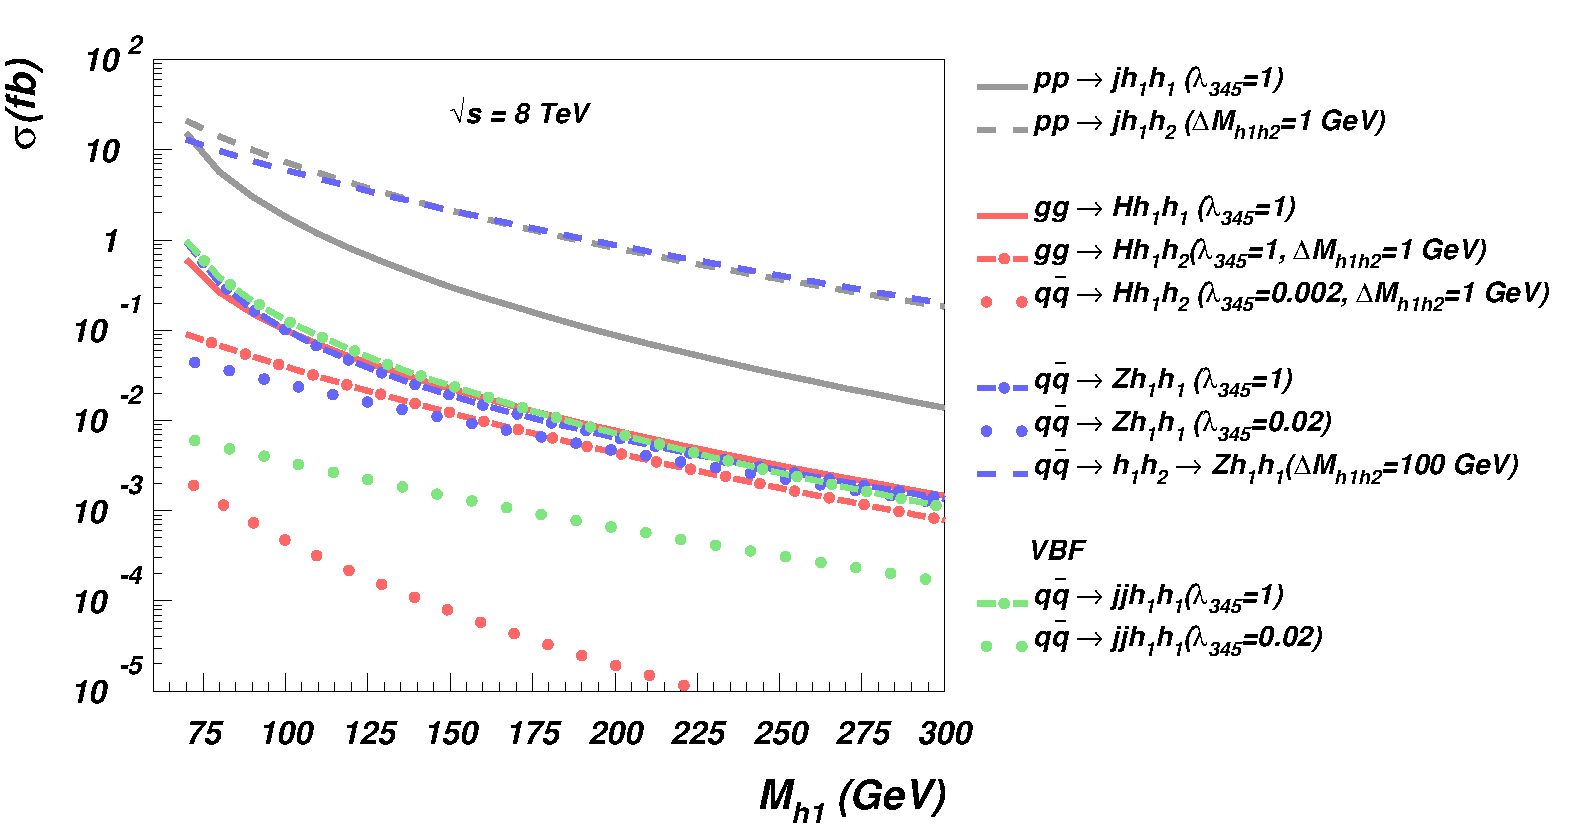
\includegraphics[height=0.4\textheight]{Figures/sigma_vs_mh1_new_8tev.pdf} 
\vskip -0.2cm
\hskip 3cm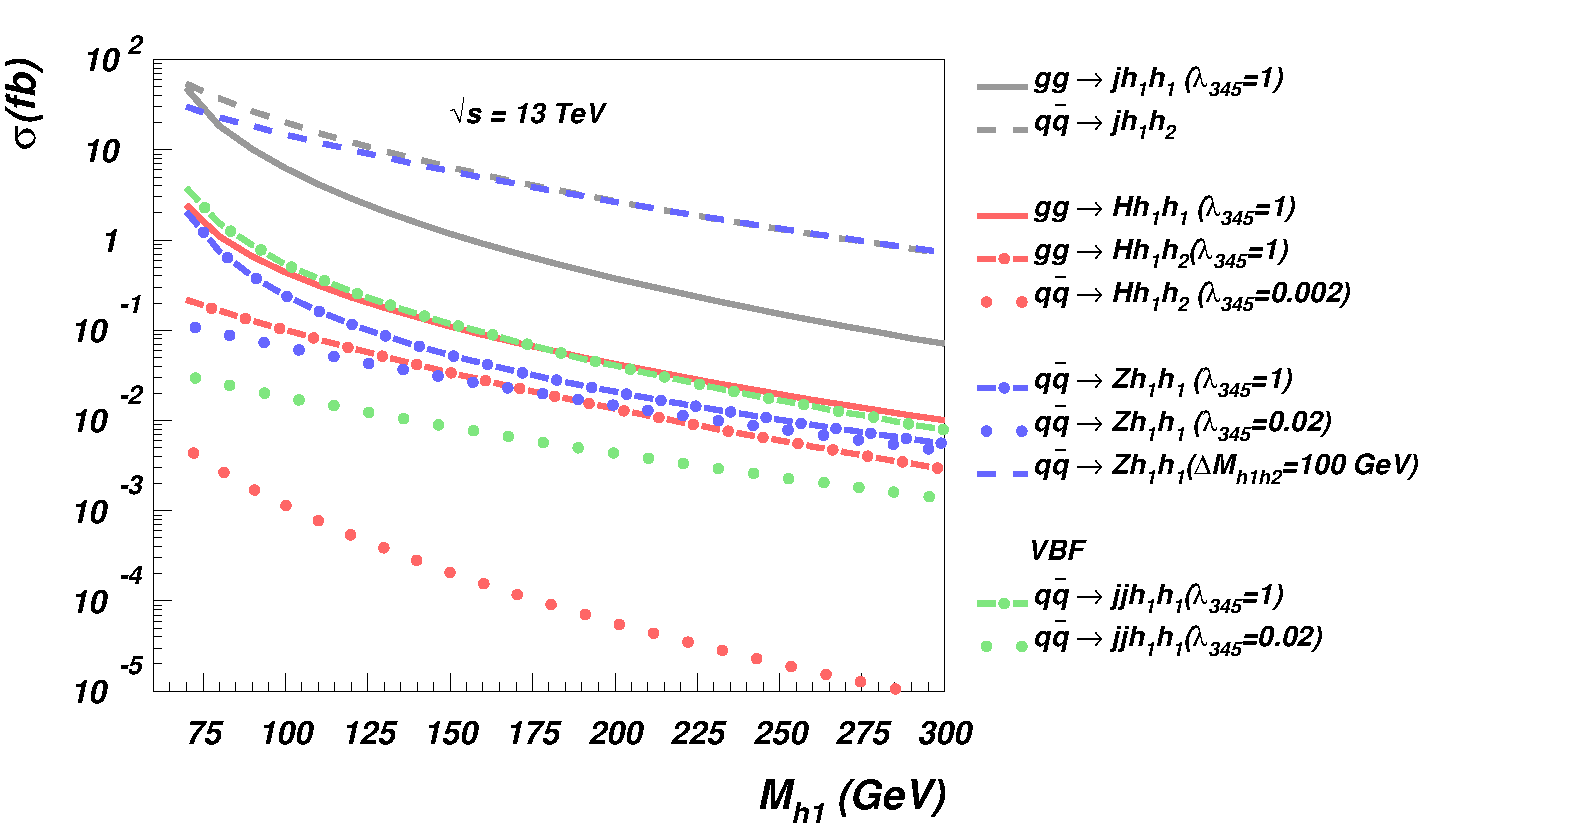
\includegraphics[trim={0 0 10.5cm 0},clip,height=0.4\textheight]{Figures/sigma_vs_mh1_new_13tev.pdf} 
\vskip -0.2cm
\caption{ Cross sections versus
Dark Matter mass, $M_{h_1}$, for  processes
contributing to mono-jet, mono-Z, mono-Higgs and VBF signatures
for the LHC@8 TeV and  LHC@13 TeV.}
\label{fig:cs}
\end{figure}
%

In Fig.~\ref{fig:cs} we present a summary of the cross sections versus
Dark Matter mass $M_{h_1}$ for all the processes mentioned above, 
which contribute to the mono-jet, mono-$Z$, mono-Higgs and VBF signatures
for the LHC at 8 and 13 TeV.
We have used the following setup for the process evaluation:
\begin{itemize}
\item the QCD renormalisation and factorisation scales $Q$ were chosen to be equal to the
transverse momentum of the pair of DM particles,  i.e. missing transverse momentum, \MET{}
for all processes;
\item the PDF and the strong coupling constant are as provided by the
NNPDF23LO (\verb|as_0119_qed|) PDF set~\cite{Ball:2012cx};
\item for all processes a cut on the minimal value of missing transverse momentum of 100 GeV 
was applied;
\item the VBF cross section has been evaluated with the following additional cuts:
  \begin{align}
    P_T^j>30\mbox{ GeV}, \hspace{2mm} \Delta\eta_{jj}>4, \hspace{2mm} E_j> 400\mbox{ GeV}.
  \end{align}
\item Below we present plots and numbers for cross sections (in the text and table)
with three significant digits corresponding to the accuracy of the MC phase space integration.
But we would like to note that when $Q$ is varied in the range $\MET/2$ to $2\times \MET$,
the QCD scale uncertainty is around 20-30\% for the tree-level cross sections presented,
dominating over PDF uncertainties which are below 10\%.
The presentation and detailed discussion of
these uncertainties is out of the scope of this paper.
\end{itemize}

For the $pp \to  h_1 h_1 j$ processes, the cross section is represented by a solid grey line 
in Fig.~\ref{fig:cs}. It was evaluated for $\lambda_{345}=1$ and scales as $(\lambda_{345})^2$.
The cross section scaling for the $gg\to  h_1 h_1 H$
processes is a bit more subtle. All diagrams except the second one in Fig.~\ref{fig:fd-mono-H1} scale as $\lambda_{345}$,
while the second one scales as  $\lambda_{345}^2$. So for large  $\lambda_{345}$ the
cross section scales as  $\lambda_{345}^4$ while for low values it scales as $\lambda_{345}^2$.
Moreover one can expect non-trivial interference between these
diagrams for negative values of $\lambda_{345}$. The cross section for this process 
evaluated for $\lambda_{345}=1$ is presented by solid red line in Fig.~\ref{fig:cs}.

The cross section for the  $pp \to h_1 h_2 j$ when $M_{h_2}-M_{h_1}=1$~GeV,
and $q\bar{q}\to h_1 h_2 \to h_1 h_1 Z$ with $M_{h_2}-M_{h_1}=100$~GeV, both of which are
independent of $\lambda_{345}$, are presented by the grey and blue dashed lines.

When $M_{h_2}-M_{h_1}=1$~GeV, the processes $q\bar{q}\to h_1 h_1 Z$ (with $h_2$ being off-shell), $q\bar{q}\to h_1 h_2 H$
and $q\bar{q}\to  j j h_1 h_1$(VBF) scale partly with $\lambda_{345}$ as discussed above.
For $\lambda_{345}=1$, a value chosen such that
the contribution from diagrams which scale with $\lambda_{345}$
is dominant, the cross section for these processes is presented 
by blue, red and green dot-dashed lines respectively.
For small values of $\lambda_{345}$ (0.002, 0.02 and 0.02 respectively), below which 
the contribution from such diagrams is less than 1\%, the cross sections are
represented by blue, red and green dotted lines.
%
Using information presented in Fig.~\ref{fig:cs}
one can easily estimate cross sections for other values of  $\lambda_{345}$ by
recalling those  cross sections which are proportional to  $\lambda_{345}^2$.

One should  stress the importance of the  $pp\to h_1 h_2j$  process 
involving $h_2$ in the final state
and the crucial dependence of the physics, i.e. the signatures and cross sections, on the mass of $h_2$:
a) in the case of a small $h_2-h_1$ mass split, this process
contributes to the mono-jet signature, which actually has a 
cross section larger than that of  $gg\to  h_1 h_1 j$
even for  $\lambda_{345}\gtrsim 1$ when $M_{h_1}> 75$ GeV;
b) when the mass split is increased to a few dozens of GeV,
the cross section of this process drops; however in this case it
produces a SUSY-like signature with soft-leptons and $\MET{}$ as studied previously and discuss above;
c) when $M_{h_2}-M_{h_1} > M_Z$,
the cross section of this process is enhanced by about two orders of magnitude
providing a mono-$Z$ signature with a rate close to that of the $pp\to h_1 h_2g$ 
process.


%\giac{[COMMENT: }{we should mention that the assumption $M_{h_2} = M_{h_1}$ is crucial here, as some processes
%involving $h_2$ depend crucially on the value of its mass.]}

%\giac{[COMMENT: }{the last diagram in Fig.12n can also be seen as a h1h2 production with decay h2->h1 Z. In this
%phase space region, the rate should be highly increased. This point is completely missed in the plot where we chose
%equal masses. Is this observation viable via a vis the constraints in the model parameter space?]}

\begin{table}[htb]
\centering
\begin{tabular}{|c||c|c|c|c|c|c|c|}
\hline
 {\bf BM}                       &  {\bf 1}  		& {\bf 2}  	   	   & {\bf 3}  		& {\bf 4}  		    & {\bf 5}     	    &  {\bf 6}  \\
  \hline\hline 
  $M_{h_{1}}$ (GeV)     	& 55      		& 55 			& 50 		      & 70		       & 100	      	      &100 \\
  \hline
  $M_{h_{2}}$ (GeV)     	& 63      		& 63 			&150  		      & 170	       	       & 105		      &105 \\
  \hline
  $M_{h_{+}}$ (GeV)   		& 150     		& 150 			&200  	  	      & 200		       & 200	     	      &200 \\
  \hline
  $\lambda_{345}$       	& $1.0\times10^{-4}$ 	 & $0.027$  		 & $0.015$ 		& $0.02$ 		& $1.0$  		& $0.002$	   \\
  \hline
  $\lambda_{2}$         	&  1.0    		& 1.0		        & 1.0	    	      & 1.0		       & 1.0		      & 1.0 \\ 
  \hline	
  $\Omega_{\rm DM} h^2$          	& $9.2 \times 10^{-2}$  & $1.5 \times 10^{-2}$   & $9.9 \times 10^{-2}$ & $9.7 \times 10^{-2}$	& $1.3 \times 10^{-4}$  &  $1.7 \times 10^{-3}$ \\
  \hline 
  $\sigma_{SI}^p$ (pb)    	& $1.7 \times 10^{-14}$ &  $1.3 \times 10^{-9}$  & $4.8 \times 10^{-10}$& $4.3 \times 10^{-10}$ & $5.3 \times 10^{-7}$  &  $2.1 \times 10^{-12}$ \\
  $R_{SI}^{LUX}$     	        & $1.6\times 10^{-5}$   &  $0.19$		 & $0.51$  		& $0.37$  		& $0.48$  		& $2.5  \times 10^{-5} $ \\
 \hline 
  $Br(H\to h_1 h_1)$     	& $5.2\times 10^{-6}$ 	&  $0.27$  		& $0.13$  		& $0.0$  		& $0.0$		 	&  $0.0$ \\
 \hline 
  $\sigma_{LHC8}$ (fb) &&&&&&\\
  ${h_1 h_1 j}$  		& $5.44\times 10^{-3}$ 	&  $288.$  		& $134.$  		& $6.05\times 10^{-3}$ 	&  $1.80$ 		&  $7.23\times 10^{-6}$ \\
  ${h_1 h_2 j}$  		& $36.7$      		&  $36.7$ 		& $6.48$  		& $3.90$ 		&  $6.93$ 		&  $6.93$ \\
  ${h_1h_1 Z}$  		& $6.14\times 10^{-2}$  &  $21.4$  		& $30.7$  		& $12.2$		&  $0.101$ 		&  $2.52\times 10^{-2}$ \\
  ${h_1h_1 H}$  		& $1.70\times 10^{-4}$  &  $8.98$  		& $4.21$  		& $2.19\times 10^{-4}$ 	&  $0.100$ 		&  $3.33\times 10^{-7}$ \\
  ${h_1h_2 H}$  		& $5.35\times 10^{-3}$  &  $6.31\times 10^{-3}$ & $9.80\times 10^{-3}$  & $7.54\times 10^{-3}$ 	&  $3.86\times 10^{-2}$ &  $5.51\times 10^{-4}$ \\
  ${h_1 h_1 jj}$		& $2.39\times 10^{-2}$	&  $17.2$  		& $8.11$  		& $4.44\times 10^{-2}$ 	&  $0.212$		&  $1.62\times 10^{-2}$ \\
 \hline 
  $\sigma_{LHC13}$ (fb) &&&&&&\\
  ${h_1 h_1 j}$  		& $1.67\times 10^{-2}$ 	&  $878.$  		& $411.$  		& $1.93\times 10^{-2}$ 	&  $6.25$ 		& $2.50\times 10^{-5} $ \\
  ${h_1 h_2 j}$  		& $92.4$      		&  $92.4$  		& $17.8$  		& $11.1$ 		&  $19.1$ 		&  $19.1$ \\
  ${h_1h_1 Z}$  		& $0.153$       	&  $46.2$  		& $66.9$  		& $28.3$ 		&  $0.241$ 		&  $6.47\times 10^{-2}$ \\
  ${h_1h_1 H}$  		& $6.69\times 10^{-4}$  &  $35.3$  		& $16.5$  		& $9.08\times 10^{-4}$ 	&  $0.441$ 		&  $1.51\times 10^{-6}$ \\
  ${h_1h_2 H}$  		& $1.18\times 10^{-2}$  &  $1.40\times 10^{-2}$ & $2.47\times 10^{-2}$  & $1.99\times 10^{-2}$ 	&  $9.82\times 10^{-2}$ &  $1.34\times 10^{-3}$ \\
  ${h_1 h_1 jj}$ 		& $0.101$	     	&  $62.7$  		& $29.6$  		& $0.189$ 		&  $0.904$ 		&  $7.49\times 10^{-2}$ \\
  \hline\hline
\end{tabular}
\caption{Benchmarks (BM) from the i2HDM parameter space
together with corresponding observables: DM relic density ($\Omega_{\rm DM} h^2$),
 spin-independent  DM scattering rate on the proton ($\sigma_{SI}^p$)
accompanied with its ratio to the experimental limit from LUX following re-scaling with the relic density: 
$R_{SI}^{LUX} =(\sigma_{SI}^p/\sigma_{SI}^{LUX})\cdot (\Omega_{DM}/\Omega_{DM}^{Planck})$,
and the LHC cross sections for mono-jet, mono-$Z$, and mono-$H$ signatures with a $\MET > 100$ GeV cut applied.
\label{tab:i2HDMbenchMarks}}
\end{table}

In Table~\ref{tab:i2HDMbenchMarks} we present
six  benchmarks (BM) from the i2HDM  parameter space
together with corresponding observables: DM relic density ($\Omega_{\rm DM} h^2$),
 spin-independent  DM scattering rate on the proton ($\sigma_{SI}^p$)
accompanied with its ratio to the experimental limit from LUX following re-scaling with the relic density: 
$R_{SI}^{LUX} =(\sigma_{SI}^p/\sigma_{SI}^{LUX})\cdot (\Omega_{DM}/\Omega_{DM}^{Planck})$.
We also present the LHC cross sections for the mono-jet, mono-$Z$ and mono-$H$ signatures
discussed above with a $\MET > 100$ GeV cut applied.
All of these benchmarks are allowed by the present experimental data.

The first two benchmarks have small and medium values of $\lambda_{345}$ and correspond to the 
scenario when $M_{h_1}$ is below $M_H/2$, and the mass split $\Delta M = M_{h_2}-M_{h_1}$ is small.
BM1 has a very small value of  $\lambda_{345}=10^{-4}$ and is therefore characterised 
by having a small $Br(H\to h_1 h_1)$ value and a very low DM direct detection rate, $\sigma^p_{SI}$,
whilst the relic density is consistent with the Planck limit {due to co-annihilation}.
The $h_1h_1j$ mono-jet signature rate at the LHC scales with $(\lambda_{345})^2$ and is therefore very low,
while the $\lambda_{345}$-independent $h_1h_2j$ signature cross section 
is about 36.7 fb (LHC@8 TeV) and 92.4 fb (LHC@13 TeV).

BM2 differs from BM1 only by the value of $\lambda_{345}=0.027$, which is chosen as the maximum value 
allowed by the Higgs invisible branching ratio. For this $\lambda_{345}$,
the $h_1 h_1 j$ mono-jet production rates are 288 fb (LHC@8 TeV) and 878 fb (LHC@13 TeV).

BM3 and BM4 correspond to the scenarios where $\Delta M > M_Z$
with $M_{h_1}$ below and above $M_H/2$ respectively,
{with the other parameters chosen such that the} relic density is consistent with Planck data.
In comparison to BM3, BM4 has a very low $h_1h_1j$ production cross section because
the SM Higgs boson is produced off mass shell.
At the same time the $h_1 h_1 Z$ cross section 
is of the same order for both benchmarks: 6.48 fb and 3.90 fb for LHC@8 TeV,
and 17.8 fb and 11.1 fb for LHC@13 TeV, respectively.

Finally, BM5 and BM6 represent the cases with a small (5 GeV) mass split and $M_{h_1}=100$~GeV.
The only difference in the input parameters is the value of $\lambda_{345}$: 
large $\lambda_{345}=1$ for BM5 and small $\lambda_{345}=0.002$ for BM6.
For both benchmarks, the DM relic density is well below the PLANCK limit, and therefore an
additional source of Dark Matter is required. Even for BM6 which has a small
value of $\lambda_{345}$, the DM relic density is
of the order of $10^{-3}$ because the DM effectively annihilate via 
$h_1 h_1 \to VV$  and $h_1 h_1 \to HH$ channels.
They are open for this value of DM mass
and are defined essentially by the weak coupling,
the contribution from $h_1 h_1 \to V_L V_L$ being small because of the small $h_1-h_2$ mass split
and the contribution from co-annihilation being subdominant for this value of mass split.
For both of these benchmarks, the $h_1 h_2 j$ channel
which has cross-sections of 6.93 fb (LHC@8 TeV) and 19.1 fb (LHC@13 TeV)
looks the most promising.

From Table~\ref{tab:i2HDMbenchMarks} one can see that different mono-object signatures are 
very complementary for these suggested benchmarks,
especially the $h_1 h_1 j$ and $h_1 h_2 j$ processes which are
the main focus of the collider study presented below.
